\articlepart{新配列のすすめ}{kouy}

\section{新配列とは?}

新配列とは、パソコンなどで日本語を入力するためのかな入力配列で、ローマ字入力とかな入力以外の配列のことです\footnote{この文章では「新配列」とはローマ字入力(QWERTYローマ字入力)とかな入力(JISかな、JIS X 6002-1980)以外のすべての配列を指すことにします。親指シフトやDvorakなどはかなり昔からある配列ですので、「新配列」という名前は違和感があるかもしれませんが、ここでは新配列に含めます。}。

パソコンで日本語を入力するときの入力方法は、多くの方がローマ字入力――キーに印刷されているアルファベットでローマ字表記を入力する方法――を使っていると思います。あるいは、かな入力――キーに印刷されているかなに従ってかなを入力する方法――を使っている方もいるでしょう。

「そもそも、かなの入力方法はその2種類しか知らない。ほかの方法なんてあるの?」と思う方も多いと思います。

しかし、日本語を入力する方法はこれ以外にも数多くあります。日本語の文章を分析して効率よく入力できるようにしたもの、覚えるのは簡単でしかも速く楽に入力できるようにしたものなど、それぞれに日本語入力がより快適になるように工夫された新配列が開発されています。

現在のパソコンは、どの配列も簡単に使うことができます。最初に覚えたのがローマ字入力だからといって、これからもローマ字入力を使い続ける必要はありません。\\

あなたも、新配列を使って快適な日本語入力環境を実現してみませんか?

\subsection{日本語を分析して作った配列}

新配列のメリットは、日本語をより効率よく入力できることです。では、なぜ新配列は効率よく入力できるのでしょうか? それは、日本語には良く出てくるかなとあまり出てこないかながあり、新配列は良く出てくるかなを打ちやすいように配置しているからです。

ローマ字入力にしろ、かな入力にしろ、あるいは新配列にしろ、最終的にはかなを入力することによって日本語を入力しています。では、かなのうち、最も入力する機会が多いかなはどれでしょうか?

図\ref{1gram}はWebサイトその他から適当に文章約100万字採集して、出現するかなの回数(漢字はかなに直して)を調べたものです。一番多く出現するのが「い」で7万4569回。次が「う」で5万9235回。3位が「ん」で5万8709回となります。出現率トップクラスのかなは5万回以上の出現回数であることがわかります。

次に下位の方を見てください。出現回数70位以下の下位グループのかなは、出現回数1000回前後のかなが並んでいます。出現率トップクラスのかなの50分の1程度の出現率です。そこまで下位でなくても、出現回数中位、例えば43位の「そ」や44位の「え」でも出現回数は1万を割っています。出現率トップクラスのかなと比べると出現率は5分の1程度しかありません。

\begin{figure*}
 \begin{center}
   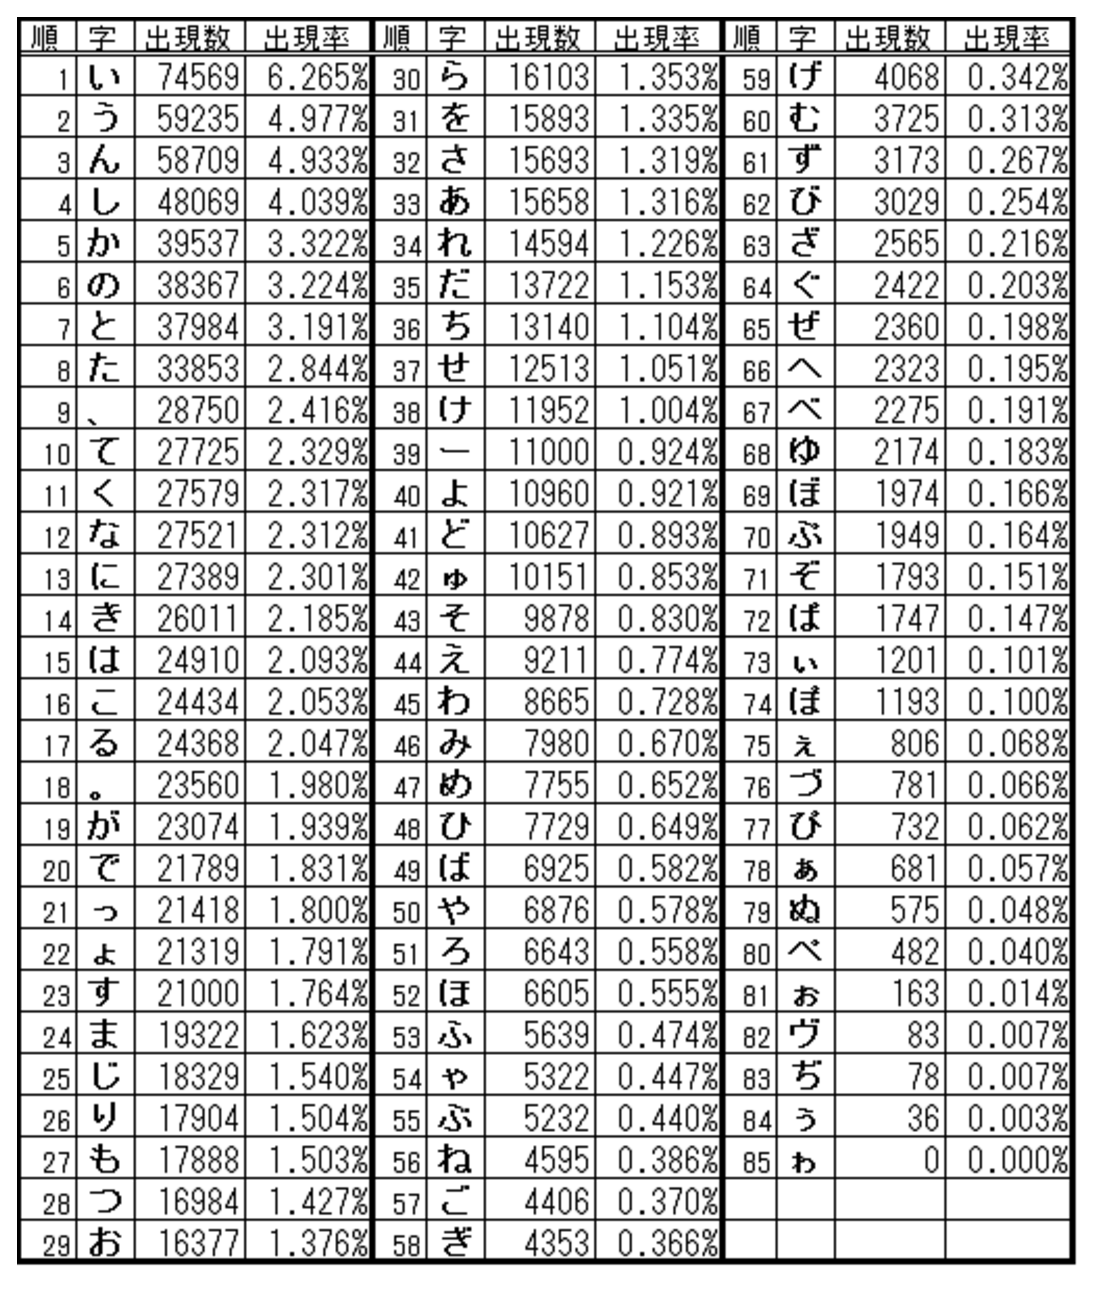
\includegraphics[width=14cm,clip]{res_kouy/1gram.eps}
 \end{center}
 \caption{文章100万字中のかな出現回数}
 \label{1gram}
\end{figure*}

このように、かなの出現率はかなによって大きく異なります。したがって、出現回数上位のかなを、キーボードの打ちやすいキーに配置すれば、効率よく入力することができるようになります。では、キーボードの打ちやすいキーはどのキーでしょうか?

キーボードのキーを打つ指は片手につき5本あります。このうち親指はキーボード最下段のキーを担当するするのでとりあえず除きます。文字キーを打つ指は人差し指、中指、薬指、小指の4本です。この中でキーを打ちやすい指はどの指でしょうか? 人差し指や中指は動かしやすく、力もあるので打ちやすい指です。逆に、小指や薬指は思うように動かせず、疲れやすいので打ちにくい指でしょう。

また、キーボードの文字キーは4段にわたって配置されています。「最上段」(キーの左から順に\key{1}\key{2}\key{3}\key{4}\key{5}……と並んでいる段)、「上段」(左から\key{Q}\key{W}\key{E}\key{R}\key{T}……)、「ホーム段(中段)」(左から\key{A}\key{S}\key{D}\key{F}\key{G}……)、「下段」(左から\key{Z}\key{X}\key{C}\key{V}\key{B}……)の4段です。このうち最も打ちやすいキーの段は、やはり指を動かさなくてすむホーム段のキーでしょう。次が1段指を動かす必要がある上段か下段。最上段は2段指を動かす必要があるので最も打ちにくい段です。

さらに、キーの横のズレや指の長さなどによって打ちやすさが変わります。図\ref{key_utiyasusa}はわたしが思う各キーの打ちやすさを示したものです。打ちやすい順に「◎、○、△、×」です。
この表の◎や○のついたキーを多く使い、△や×のついたキーをあまり使わないようにすれば、効率よく入力することができます。


\begin{figure*}
 \begin{center}
   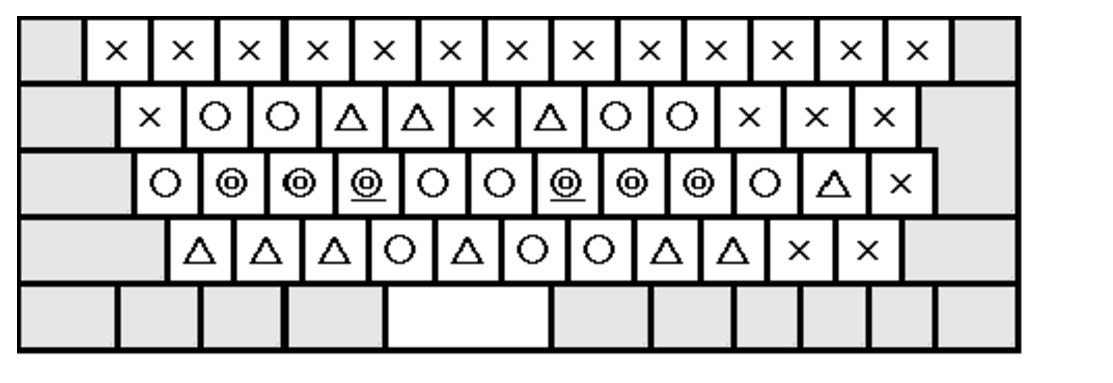
\includegraphics[width=14cm,clip]{res_kouy/key_utiyasusa.eps}
 \end{center}
 \caption{各キーの打ちやすさ}
 \label{key_utiyasusa}
\end{figure*}

このように、新配列は日本語とキーボードを分析して作ります。新配列で考慮する要素を“文字の出現率”と“キーの打ちやすさ”という2種類を紹介しましたが、他にも2文字以上で連続して出現することが多い連なり(例えば、「ょう」「てい」「かい」などは出現率が高い)や、良く出現するフレーズ(「ます。」「という」などは出現率が高い)も考慮します。また、1キーでの打ちやすさのほかに、連続してキーを打つ場合の打ちやすさも考慮します(例えば、\key{K}\key{J}というキーの連続は非常に打ちやすい。\key{M}\key{U}のように同じ指で遠いキーを続けて打つキーの連続は打ちにくい)。

図\ref{dakensuu_ro-maji}~\ref{dakensuu_keinarabe}は、図\ref{1gram}のデータを使用して、1万字(かなで数えて)の文章を入力した場合に各キーを何回打鍵するかを配列別に示したものです\footnote{図中のキーボード外の数字の意味:下の上段は小指・薬指・中指・人差し指の打鍵数、下の下段は上段の合計、右は最上段・上段・中段・下段の打鍵数、右下の上段は通常のシフトや同時打鍵シフトを0打鍵と数えた場合の打鍵数、右下の下段は通常のシフトや同時打鍵シフトを1打鍵と数えた場合の打鍵数。}。図を見ていただくと、図\ref{dakensuu_ro-maji}(ローマ字入力)、図\ref{dakensuu_JIS-kana}(かな入力)に比べ、図\ref{dakensuu_NICOLA}~\ref{dakensuu_keinarabe}の新配列3種(親指シフト、月配列、けいならべ)はホームポジションのキーを多く使うのがわかると思います。

日本語で良く出てくる文字を打ちやすいキーで入力できる。だから新配列は打ちやすいのです。

\begin{figure*}
 \begin{center}
   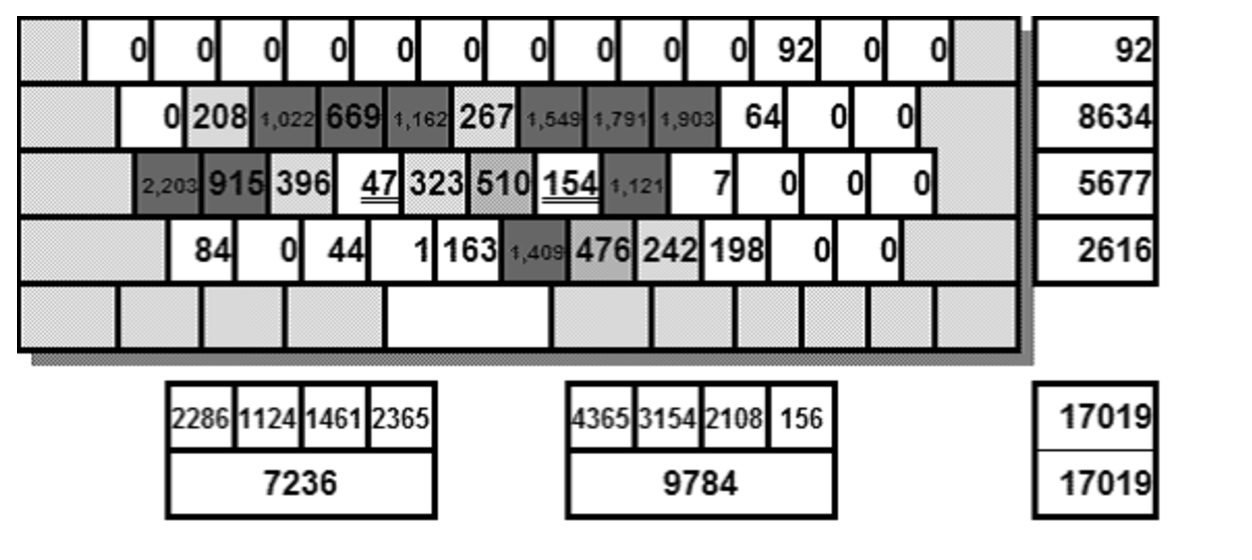
\includegraphics[width=14cm,clip]{res_kouy/dakensuu_ro-maji.eps}
 \end{center}
 \caption{1万字の文章を入力した場合の打鍵数 ローマ字入力}
 \label{dakensuu_ro-maji}
\end{figure*}

\begin{figure*}
 \begin{center}
   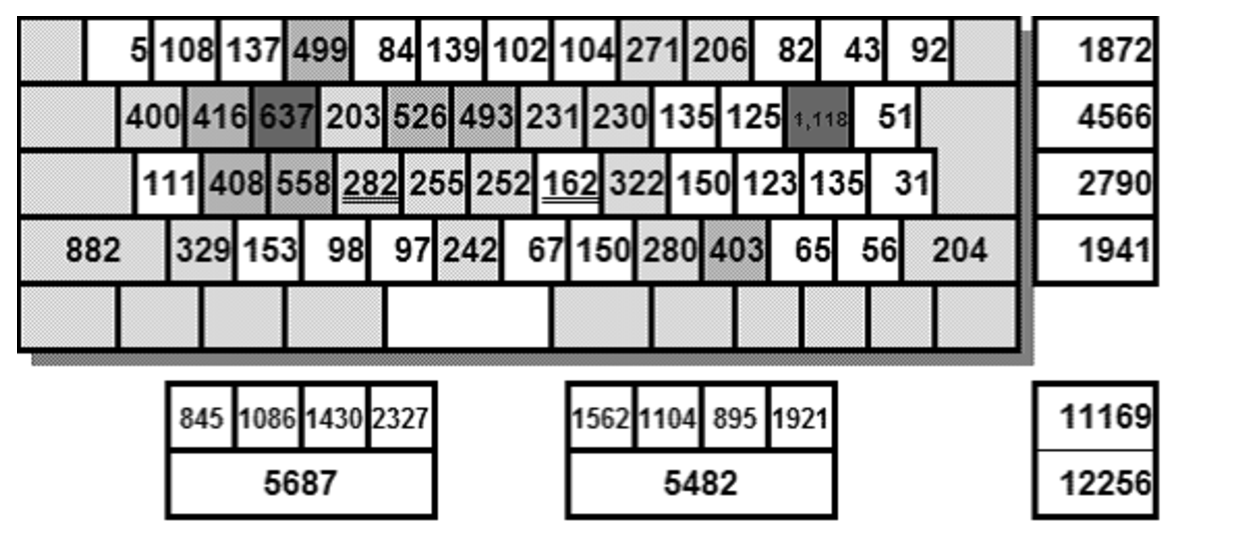
\includegraphics[width=14cm,clip]{res_kouy/dakensuu_JIS-kana.eps}
 \end{center}
 \caption{1万字の文章を入力した場合の打鍵数 かな入力}
 \label{dakensuu_JIS-kana}
\end{figure*}

\begin{figure*}
 \begin{center}
   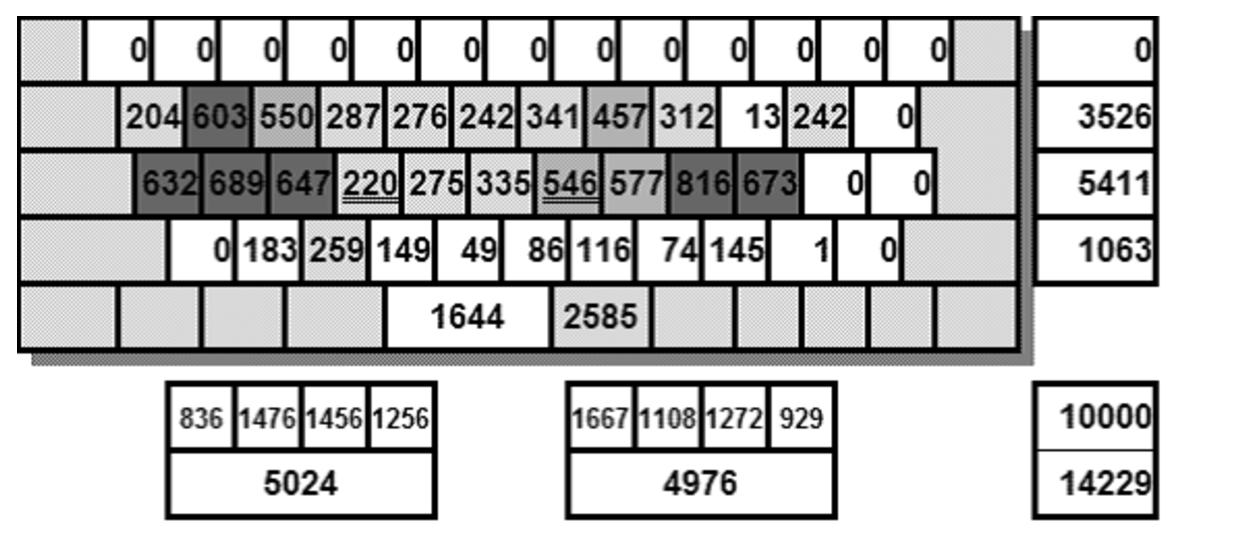
\includegraphics[width=14cm,clip]{res_kouy/dakensuu_NICOLA.eps}
 \end{center}
 \caption{1万字の文章を入力した場合の打鍵数 親指シフト(NICOLA)}
 \label{dakensuu_NICOLA}
\end{figure*}

\begin{figure*}
 \begin{center}
   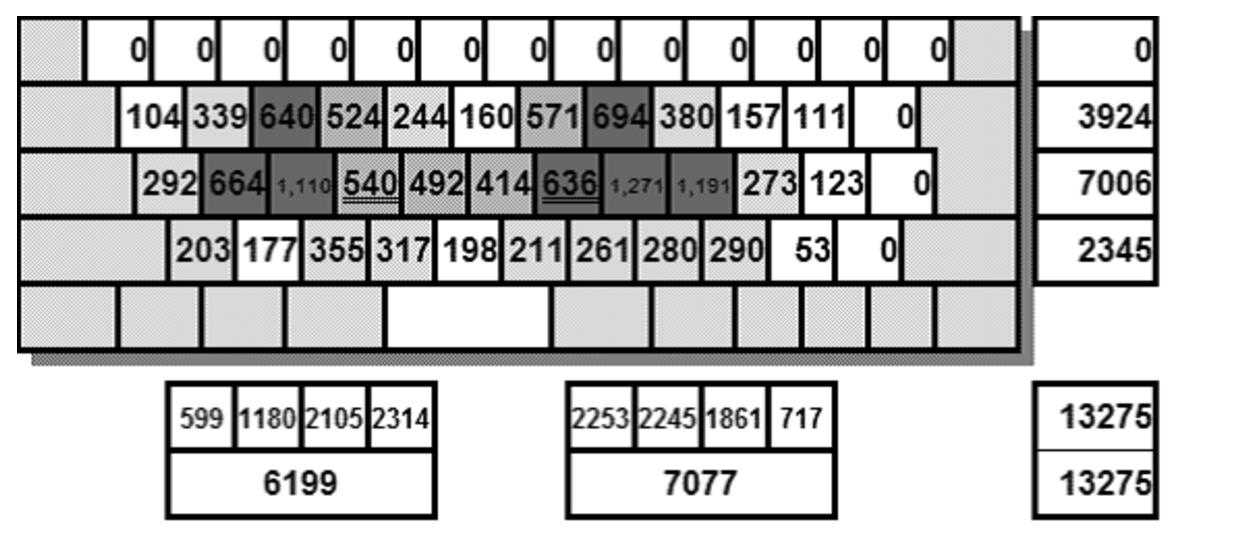
\includegraphics[width=14cm,clip]{res_kouy/dakensuu_tuki2-263.eps}
 \end{center}
 \caption{1万字の文章を入力した場合の打鍵数 月配列2-263式}
 \label{dakensuu_tuki2-263}
\end{figure*}

\begin{figure*}
 \begin{center}
   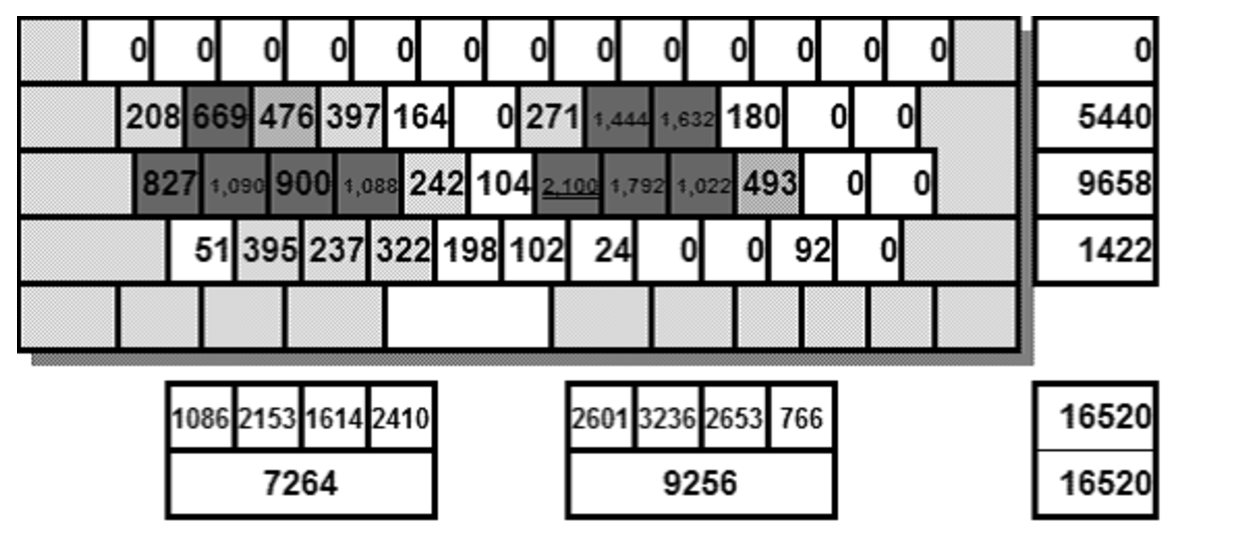
\includegraphics[width=14cm,clip]{res_kouy/dakensuu_keinarabe.eps}
 \end{center}
 \caption{1万字の文章を入力した場合の打鍵数 けいならべ}
 \label{dakensuu_keinarabe}
\end{figure*}

\section{なぜ今、新配列か?}

新配列が優れていると言っても、もうパソコンもインターネットも日常的に触れる世の中。ローマ字入力に慣れていて何の不都合もなく使っているのに、今さら新配列なんて……と思う方もいるかもしれません。

しかし、パソコンとインターネットが普及した今だからこそ、新配列は誕生し、使いやすくなったと言えるのです。「今さら新配列」ではなく「今こそ新配列」なのです。

\subsection{いま使っているパソコンで新配列を使えるようになった}

1980年代から1990年代にかけて、パソコンが普及する前に、ワープロ専用機が普及していた時代がありました。ワープロ専用機の時代の配列の選択は、そのワープロに搭載されている配列を使うしかありませんでした。多くのワープロではローマ字入力とかな入力しか搭載されていませんでしたので、使用できる配列は事実上この2種類に限定されていたのです。

当時もローマ字入力とかな入力以外に、親指シフト(NICOLA)や新JIS配列といった「新配列」は存在していました。しかし、親指シフトを使おうと思ったら富士通のOASYSを、新JIS配列を使おうと思ったらそれが搭載されている一部の機種を購入するしかありませんでした。ましてや、自分でオリジナルの配列を作るなど夢物語だった時代です。

現在なら、購入時そのパソコンに使いたい新配列が搭載されていなくても、あとから追加して実装することができます。

配列を実装するソフトウェアを使用すると、今使っているパソコン、今使っているキーボードのままで新配列を使用することができます。このような新配列を実装するソフトウェアのことを「配列エミュレータ」と呼びます(以下、単にエミュレータとも書きます)。エミュレータはさまざまな種類の物があり、無料で使うことができるものもあります。また、インターネットを通してダウンロードできるので、だれでも簡単に入手できます。さらに、一部の新配列は、エミュレータを使うまでもなく、IMEを使って実装できたり、OSに最初から搭載されているものもあります。

新配列を導入するためのハードルは、昔に比べはるかに低くなったのです。

\subsection{多様な配列が生まれている}

パソコンとインターネットにより新配列が受けた恩恵は、これだけではありません。

前述の通り、現在ではエミュレータを使えば簡単に新配列を実装することができます。そしてエミュレータの多くは、文字の配置を自由に入れ替えられるという機能を備えています。この機能により、かつては夢物語だった「自分でオリジナルの配列を作る」ことができるようになりました。「こうすればもっと良くなる」と思う点を修正したり、一からまったく新しい配列を作るということが、簡単にできるようになったのです。

これにより、2000年前後から現在にかけて、数多くの新配列が生み出されるようになりました。多くは個人によって作られたものですが、インターネット時代らしく、ネット上に公開され、多くの人の意見を取り入れて少しずつ修正して作られた新配列もあります。

新配列を作るには、先にも書いた通り日本語の分析が不可欠です。かつては、日本語の文章を採集して、それを解析するというのは大変な手間がかかる作業でした。

しかし、これさえもパソコンとインターネットが解決してしまいました。現在では、配列を作るために必要な日本語のデータはインターネット上で公開されています。かつては個人ではとても手に負えなかったようなデータを、簡単に手に入れることができるのです。さらに必要なら、自分で日本語を分析することもできます。そのために必要な文章解析ツールも、ネットからダウンロードできるのです。

あらたな新配列が次々と誕生したことにより、新配列の選択肢は大きく広がりました。かつてはローマ字入力やかな入力以外の配列と言えば、親指シフトくらいしか選択肢がありませんでした。現在では、親指をシフトとする配列、中指をシフトとする配列、同時打鍵を使う配列・使わない配列、覚えやすさに重点を置いた配列など、それぞれに優れた特徴のある配列が多数生み出されています。21世紀に入ってから10年以上が経ち、新配列はまさに\ruby{百花繚乱}{ひゃっかりょうらん}。そろそろ主要なアイデアも出尽くし、円熟期を迎えたと言えると思います。

今なら、あなたが気にいる新配列がきっと見つかるはずです。

\section{今なら新配列だって覚えられる}

新配列が台頭してきたのはわかったけれど、すでにローマ字入力に慣れているし、いまさら入力方法を変える気にはなれない、と思う方も多いかもしれません。

初めてパソコンを触ったとき、キーボードの入力に苦戦した記憶は誰にでもあると思います。どこに何のキーがあるのかまったく分からない。1文字入力するごとにキーボードから目的のキーを一つ一つ探し出す。「こんにちは」と1語入力するだけでも一苦労。新配列を使うとすると、またあの経験を繰り返さなければならないのか。もうあんな苦労はまっぴら御免、と思う気持ちもわからないではありません。

しかし、確かに新配列を使いこなすには一定の練習が必要ですが、新配列の習得はそれほど大変なことではありません。初めてパソコンに触れたときにローマ字入力を覚えたときと比べれば、ずっと簡単に覚えることができます。

\subsection{キーボードに慣れている}

新配列の習得が簡単な第一の理由は、すでにキーボード自体には慣れているということです。みなさんはローマ字入力なりかな入力なりで、キーボードで文字を入力するということ自体は――それぞれに程度の差はあるでしょうが――習得されていると思います。

パソコンに触れた当初、キーボードに初めて触れたときに文字入力に苦労したのはなぜでしょうか? もちろん、どのキーがどこに配置されているか分からないという理由もあるでしょう。しかし、キーボード自体に慣れていないことが大きな理由だったはずです。押そうとしているキーを目で見て、位置を確認しないとそのキーを押せない。キーボードを見ないで打とうとしても、どの指をどのくらい動かせばどのキーを押せるのか、どのくらいの強さで押せばいいのか、まったく見当がつかない。押したつもりで押せていなかったり、押していないはずののキーが押されていたりする。うっかりするとキーの間に指が入って2つキーを押してしまう……。最初はそんな状態だったと思います。

キーボードに慣れた今なら、そんなことはありません。キーボードに対する感覚はすでに身についています。どのキーを打てばいいのか分かれば、目的のキーを打つことは簡単にできます。その感覚は新配列でもそのまま使うことができます。

さらに、すでにパソコンの操作に慣れているという理由もあります。パソコンに触れた当初は、どのキーを押したら何が起こるのか予測できない状態です。1つキーを押し間違えただけで致命的な事態が起こるかもしれない。間違ったキーを押したとき、どうすれば修正できるのかもわからない。だから間違えたくない。すると、いちいち確認しないとキーを押せないし、いったん間違えると修正に時間がかかります。これではなかなか入力が進まず、なかなか慣れることができません。

今ならそんなことはありません。とりあえずカチャカチャと入力して、間違っていたら直せば良いだけのことです。どんどんキーを打ってどんどん修正していけば、すぐに慣れることができます。

初めに配列を覚えたときというのは、実は配列以外のことも同時に覚えていたのです。今なら、キーボードには慣れているし、パソコンの操作も分かります。配列を覚えることだけに集中できるのです。

\subsection{打ちやすいキーを多く使う}

新配列の習得が簡単なもう一つの理由は、新配列は打ちやすいキーを多く使うということです。キーボードのキーの中には、打つのが簡単なキーと難しいキーがあります。打つのが簡単なキーを多く使うほど習得しやすくなります。

では、打つのが簡単なキーとはどのキーでしょうか? ホームポジションではないキーを打つ場合は、指をそのキーの上に正確に動かさなければいけませんから、打つのが難しくなります。また、小指は力が弱くほかの指に比べて使いにくいので、正確にキーを打つのが難しい指です。逆に、指をキーの上から動かさずに済むホームポジションのキーを、動かしやすい人差し指・中指・薬指を使って打つ場合は、簡単に打つことができます。
よって、最も打つのが簡単なキーは、人差し指・中指・薬指のホームポジションのキー、具体的には\key{S}\key{D}\key{F}、\key{J}\key{K}\key{L}の6キーとなります。

しかし、ローマ字入力ではこれらのキーの使用率はあまり高くありません。ローマ字入力で最もよく使うキーは、母音キー、すなわち\key{A}\key{I}\key{U}\key{E}\key{O}の5キーです。この5キーは、先ほど挙げた打つのが簡単な6キーには一つも含まれていません。つまりローマ字入力は、打つのが簡単なキーをあまり使わず、それより打つのが難しいキーを頻繁に使う配列なのです。これでは習得が難しくなるのも必然です。

かな入力も、打つのが簡単なキーを多く使うとは言えない配列です。ホーム段より上段の方が使用率が高かったり、最上段にも使用率がかなり高いキーがあったり、圧倒的に出現率が高い濁点がホームポジションから外れた、しかも小指が担当するキーに配置されていたりします。指がホームポジションから離れて遠くのキーを打ちに行く機会が多いのですから、複雑な指の動きも増え、難度もアップします。

指を動かさなくて済むホームポジションのキーを多く使い、同じ指で異なるキーを続けて打つような複雑な動作はできるだけしない。そんな配列なら、習得するのはもっと簡単なことになります。

新配列は、日本語で多く出現する文字を入力しやすいように配置しています。必然的に、打ちやすいキーの使用率が高くなり、複雑な指の動きも少なくなります。これは入力をより効率的にできるように工夫した結果ですが、そのような配列は――習得した後に効率的に入力できるだけでなく――習得すること自体も易しくなるのです。

\section{新配列FAQ}

\subsection{新配列をいま使っているパソコンで使える?}

\subsubsection*{【質問】}

新配列を使うには、新たにパソコンやキーボードなどを買う必要があるのですか? 新配列をいま使っているパソコンで使うにはどうしたらよいですか?

\subsubsection*{【回答】}

配列やOSによってさまざまな実装方法がありますが、配列エミュレータと呼ばれるソフトウェアを使って新配列を実装するのが簡単な方法です。エミュレータを使えば、いま使っているパソコン、キーボードを使用したまま新配列を使用することができます。新たにパソコンやキーボードを購入する必要はありません。

エミュレータはさまざまな種類のものが存在します。以下に代表的な配列エミュレータを挙げます。

\begin{itemize}
 \item 『姫踊子草』(シェアウェア)
 \item 『DvorakJ』(フリーソフト)
 \item 『やまぶき』(フリーソフト)
\end{itemize}

また、配列エミュレータのほかに、キーカスタマイズソフト(キーバインド変更ソフト)と呼ばれるジャンルのソフトもあります。配列エミュレータが主にキーを押したときに入力される文字を変更するのに対し、キーカスタマイズソフトはキーの機能そのものを変更します。ただし、配列エミュレータでキーの機能を変更できたり、キーカスタマイズソフトでも入力される文字を変更できるものもあるので、その境目はあいまいです。以下、代表的なキーカスタマイズソフトを挙げます。

\begin{itemize}
 \item 『のどか』(シェアウェア)
 \item 『Yet Another Mado tsukai no Yuutsu』(フリーソフト)
 \item 『窓使いの憂鬱』(フリーソフト)
 \item 『KeySwap for XP』(フリーソフト)
 \item 『KeyRemap4MacBook』(フリーソフト)
\end{itemize}


\subsection{ほかのパソコンを使う時に困らないですか?}

\subsubsection*{【質問】}

新配列を使うにはエミュレータなどを使用する必要があるそうですが、そうすると自分のパソコンを使うときはよいですが、ほかのパソコンを使うときに新配列を使うことができないのではないですか? それは困りませんか?

\subsubsection*{【回答】}

新配列を実装するにはエミュレータなどを使用する必要がありますが、エミュレータはUSBメモリなどに入れて持ち運べるタイプのものもあります。それを利用すれば、どのパソコンでも新配列を利用することは可能です。

また、新配列を使えない状況では、そのときだけローマ字入力を使用することにすれば問題ありません。次のFAQをご覧下さい。

\subsection{ローマ字入力と新配列を併用できますか?}

\subsubsection*{【質問】}

新配列を覚えても、ローマ字入力を使うことはできますか? ローマ字入力を忘れてしまうことはありませんか?

\subsubsection*{【回答】}

新配列を覚えても、いままで使っていたローマ字入力はそのまま使うことができます。一度自転車の乗り方を覚えると、しばらく自転車に乗らない期間があっても乗り方は忘れない、という現象に似ています。

実際、新配列を使っている人の多くは、必要があればローマ字入力で入力しています。わたしも自分のパソコン以外で入力する必要があるときはローマ字入力を使用していますが、まったく問題なく使用できます。

\subsection{ローマ字入力はアルファベットの配置を使えるから良いのでは?}

\subsubsection*{【質問】}

パソコンの文字入力では、かなの入力のほかにアルファベットの入力も使います。ローマ字入力ならアルファベットの配列1つでかなもアルファベットも入力できるので、やはりローマ字入力を使うのが合理的ではないでしょうか?

\subsubsection*{【回答】}

ローマ字入力の習得を通じてアルファベットの配置もある程度覚えることができますので、パソコン初心者の段階、つまりかなの入力もアルファベットの入力も覚えいてないという段階では、確かにメリットはあると思います。初めてパソコンに触った人がローマ字入力を覚えるというのは、一定の合理性があると思います。

しかし、それ以上の段階になると、ローマ字入力を通じてアルファベットの入力を練習できるという効果はほとんど無くなってきます。ローマ字入力に慣れてくると、ローマ字入力をする際でもアルファベットをほとんど意識しないで入力できるようになります。「か」と入力するときに、\key{K}と\key{A}を打つと意識するのではなく、単に「か」の入力に必要な2つのキーを打つという感覚になります。アルファベットを意識しないのですから、ローマ字入力を使い続けても、アルファベットの入力が上達することはありません。英語入力は英語入力で、ローマ字入力とは別に習得する必要があります。

よって、アルファベットの入力を使うとしても、ローマ字入力が有利ということはありません。かなの入力方法はアルファベットの入力とは切り離して、あくまで“かなの入力”をしやすい方法を選ぶ方が合理的だと思います。

\subsection{新配列を覚えるのにどれくらいの時間がかかりますか?}

\subsubsection*{【質問】}

新配列を使ってある程度すらすら入力できるようになるまで、どれくらいの時間がかかりますか?

\subsubsection*{【回答】}

練習方法や、どれくらい集中して練習できるか、覚える新配列の難度などによって異なりますが、これまでの新配列を覚えた人の体験談によると2週間~2か月ほどのようです。

新配列を習得するまでは、大きく2つのステップに分かれます。1つ目が「頭のステップ」――配列図を頭の中に入れる――、2つ目が「指のステップ」――ある文字を入力しようと思ったときに指が瞬時にそのキー打てるようになる――、です。「頭のステップ」にかかる期間は配列によって大きく異なります。五十音順に並べたような単純な配列ならすぐにでも覚えられるでしょう。覚える要素が多くなるほど覚えるのが難しくなります。個人個人の記憶力や練習の集中度によっても異なるでしょう。「指のステップ」に関しては、配列の差はそれほどありません。単純な配列であっても指がすぐ動くなるようになるまでにはある程度の練習が必要です。こればかりはとにかく使って慣れるしかないようです。

最初は指が動かなくて苦労すると思いますが、少し入力速度が上がれば同じ練習時間で今までより多くの練習ができることになます。すると練習効率が良くなり、その結果入力速度が上がって、さらに練習効率が良くなり……と加速度的に入力速度が上がっていきます。こうなれば新配列習得間近と言えるでしょう。

新配列を覚えるコツを一つ。新配列では良く出現するかなは打ちやすいキーに配置されています。したがって、良く出現するかなを探すときは打ちやすいキー、あまり出現しないかなを探すときは打ちにくいキーを探すと見つかりやすくなります。

どのかなが良く出現するのか――先に掲載した図1-1の通りですが――分からないと思うかもしれません。おおざっぱに言うと、五十音表の最初の方に出てくるかなは良く出てきます(ただし、「ん」は最頻出かなの一つです)。もう少し詳しく書くと、あ行~た行はほぼすべて出現率上位のかなです。な行は「な」「に」と「の」、は行は「は」だけ。このくらいまでが出現率が高いと言えるかなです。例外はありますが、これだけでも新配列を覚える助けにはなると思います。

\subsection{新配列の練習方法はどうすればよいですか?}

\subsubsection*{【質問】}

新配列の練習はどのような方法で行えばよいでしょうか?

\subsubsection*{【回答】}

個人個人で好みや環境、練習にかけられる時間などが異なりますので、ベストの方法はそれぞれ異なると思います。ここではわたしがおすすめする方法を一つ紹介します。

まず、配列図を暗記します。この段階では実際にパソコンを使った文字入力はしません。配列図を紙に書いて持ち歩いて、空き時間にときどき見るようにすると覚えやすいと思います。配列図を何も見ずに紙に書けるくらいまで覚えるとベストです。ただし、配列図を左から順番に読んで覚えるようなやり方で覚えてもあまり意味がありません。かなとキーを1対1で覚えるように心がけてください。

配列図を覚えたら、タイピングゲームで練習します。『タイプウェル』は記録が詳細に残って自分の成長を確認できるのでおすすめです。まだ実際の文章入力では使用しません。文章を考えるというのは大変な作業です。まだ1文字1文字入力するのも大変な段階ですから、文章を考えながら新配列の練習もするというのは、大変な作業を同時に行うことになり、輪をかけて大変な作業になります。タイピングゲームなら入力する文字はゲームの方で自動的に提示してくれますので、自分は配列の練習に集中することができます。

この際、配列図を完全に覚えきるまでは、配列を書いた紙をディスプレイの近くに貼っておくと良いでしょう。ただし、入力できると思ったら紙を見ないでキーを押してください。覚えているのに紙を見てしまうと、入力速度に自分でブレーキを掛けてしまうことになり、成長に水を差します。とりあえずキーを打って、間違っていたら修正すればよいのです。

そしてある程度の速度で入力できるようになったら――タイプウェルで言えば総合レベルEくらい――実際の文章入力でも使用し始めます。

いま紹介した練習方法はあくまで一例です。「思い立ったその日から即実戦投入!」という練習方法もあります。それぞれで良いと思う方法を選んでください。

また、練習用ソフトや練習用テキストが用意されている新配列もあります。例えば、親指シフト(NICOLA)には、『親指シフト練習』という練習用のフリーソフトがあります。これらを利用するのも良いでしょう。

\subsection{習得するまでの間、日常の文章入力作業をどうすればよいでしょうか?}

\subsubsection*{【質問】}

新配列を習得するまでの間、文章入力速度が著しく低下するのが苦痛です。どうしても近いうちに書き上げなければいけない文章もあります。どうすればよいですか?

\subsubsection*{【回答】}

ある程度集中して練習できる期間があればベストですが、実際には難しい場合も多いと思います。わたしの意見では、まだ新配列での入力速度では実際の文章入力で使うには不足だという場合は、無理してまで練習中の新配列を使用しないで、ローマ字入力で入力しても良いと思います。ローマ字入力を使用したからといって新配列の練習効果が著しく落ちるということはありません。

もちろん、実際の文章入力をする必要がない、新配列の練習に集中できる期間を確保できるならそれが理想です。正月休みなどを利用するのも一つの方法でしょう。

\section{おすすめ新配列}

それでは新配列がどのようなものなのか具体的に見ていきましょう。新配列は実装環境、習得難度、配列理論などにより、数多くの種類があります。ここではわたしがおすすめする新配列を5つ紹介します。

\subsection{親指シフト(NICOLA)}

親指シフトは新配列の中で最も有名な配列です。ワープロ専用機の時代から存在する配列で、現在でも多数の愛用者がいます。

\begin{figure*}
 \begin{center}
   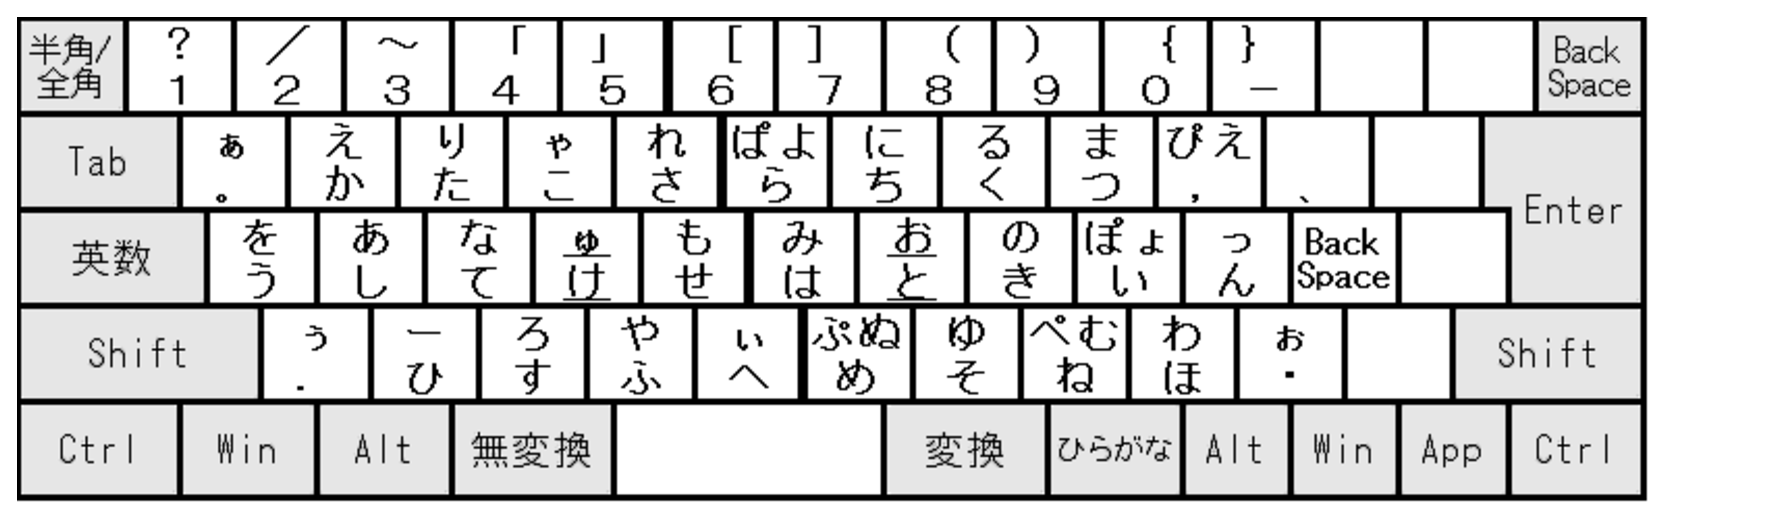
\includegraphics[width=14cm,clip]{res_kouy/NICOLA.eps}
 \end{center}
 \caption{親指シフト(NICOLA)配列図}
 \label{NICOLA}
\end{figure*}

\subsubsection*{親指をシフトキーにする}

親指シフトの最大の特徴は、「親指キー」を使用して文字を入力することです。

図\ref{NICOLA}は親指シフトの配列図です。1つのキーに2つの文字が書かれています。キーの下側に書かれた文字は、単にそのキーを押すことによって入力します(単打)。そしてキーの上側の文字は、そのキーを押す手と同じ手の「親指キー」(通常は\key{無変換}か\key{スペース}か\key{変換}のいずれか。あとで詳しく説明します)を同時に押すことによって入力します。例えば、上段の左から2番目のキー(\key{W})には「か」と「え」という2種類のかなが書かれています。「か」と入力するときは、\key{W}を単に押します。「え」と入力するときは\key{W}と\key{左親指}を同時に押します。また、そのキーを押す手と反対の手の親指キーを同時に押した場合は、単打で入力できるかなに濁点が付いた文字を入力します。例えば\key{W}と\key{右親指}を同時に押すと、「が」が入力されます。このように、親指シフトではシフト側の文字を入力するときに、親指キーを使用します。

日本語入力の際、親指担当のキーはあまり使われることのないキーです。漢字変換のときはある程度使用しますが、その他の操作は使用率はそれほど高くありません。英語の場合ですとスペースは非常に良く入力するので親指も使うのですが、日本語の文章ではスペースはあまり使いません。これでは指の能力を十分に活用できているとは言えません。親指を文字入力に使用することで、指の能力をフルに活用することができるようになります。

\subsubsection*{同時打鍵とはどういう意味か?}

先ほど「\key{W}と\key{左親指}キーを“同時に”押します」と書きました。親指シフトでは親指キーと文字キーを「同時に」打鍵するというのも大きな特徴です。「同時に打鍵する」というと何やら難しい操作方法のように聞こえます。少しでも押すタイミングがずれたら入力できないのか、そんな風に想像される方もいるかもしれません。

しかし、同時打鍵という言葉の意味は「どちらのキーを先に押しても構わない」ということです。普通のシフト(通常小指で押す\key{Shift}で行うシフト)の場合は、キーを押す順番は決まっています。例えばアルファベットで(大文字の)「A」と入力する場合、通常は\key{Shift}を押してから\key{A}を押します(さらに、\key{A}を押すまでは\key{Shift}を離してはいけません)。この順番は必ず守る必要があります。\key{A}を押した後に\key{Shift}を押すという操作で入力することはできません。

同時打鍵の場合はこの順番の制約がありません。「え」と入力する場合は\key{W}と\key{左親指}キーを押しますが、この2つのキーはどちらを先に押しても構いません。\key{W}、\key{左親指}の順番で押しても良いですし、\key{左親指}、\key{W}の順番で押すこともできます(2つ目のキーを押すまで1つ目のキーを離してはいけません)。したがって、「同時打鍵」という言葉から連想されるような厳密なタイミング合わせは必要はありません。だいたい同じタイミングでキーを押せば同時打鍵と判定されます。

同時打鍵により、2つのキーを押す操作でありながら、1つのキーを押すのと同じタイミングで文字を入力することができます。普通のシフトであれば「\key{Shift}を押してから\key{A}を押す」というように、2つのキーを2回のタイミングで押す必要があります。同時打鍵なら「\key{W}と\key{左親指}を同時に押す」というように、2つのキーを押すにもかかわらず、キーを押すタイミングは1回しかありません。押すキーの数が増えても、キーを1回押すタイミングで次々と文字を入力できる。この感覚は同時打鍵ならではのものです。

\subsubsection*{普通のキーボードで親指シフトができる?}

先ほどから再三「親指キー」という言葉が出てきています。しかし、普通のキーボードには、当然ながら「親指キー」というキーは存在しません。もともと親指シフトは、専用の親指シフトキーボードを使うことを前提としています。図\ref{oyayubi-shift_keyboard}が親指シフトキーボードです。キーボードの下の方、通常親指が担当する段の中央付近に\key{左親指}と\key{右親指}という2つのキーが存在します。親指シフトキーボードは現在も販売されています。親指シフトキーボードを搭載したノートパソコンもあります。親指シフトを使う場合は、これらのキーボードを使用するのが本来の使い方です。しかし、親指シフトキーボードは1万円~数万円しますので、初めて親指シフトを試そうという人にとっては、ちょっとハードルが高いかもしれません。


\begin{figure*}
 \begin{center}
   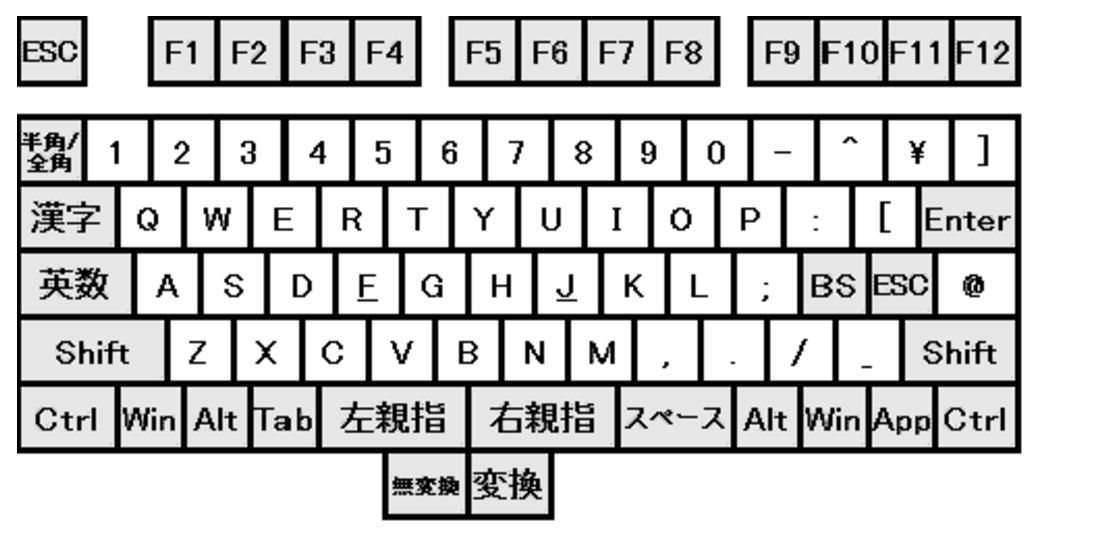
\includegraphics[width=14cm,clip]{res_kouy/oyayubi-shift_keyboard.eps}
 \end{center}
 \caption{親指シフトキーボード}
 \label{oyayubi-shift_keyboard}
\end{figure*}

でもまだ親指シフトをあきらめる必要はありません。現在では普通のキーボードを使って親指シフトをすることができるのです。配列エミュレータを使えば、キーボードの最下段にある\key{無変換}、\key{スペース}、\key{変換}のどれか2キーを親指キーとして、あたかも親指シフトキーボードのように使うことができます。例えば、\key{スペース}を\key{左親指}、\key{変換}を\key{右親指}であるかのように扱って、親指シフトを実装することができるのです。

「親指キーにしたキーを元々のキーの機能を使いたい場合はどうすればいいのか?」という疑問がわきますが、エミュレータの方で「文字キーと同時に押した場合はシフトキーとして、文字キーを押さずに離した場合はもともとのキーとして」処理してくれます。例えば、\key{スペース}を\key{左親指}にした場合でも、\key{スペース}を単に押して離した場合は、普通に\key{スペース}を押したものとして扱ってくれます(そのようにしないで親指シフト専用のキーとすることもできます)。

どのキーを親指キーにするかは、いくつかの方法があります。《\key{スペース}を\key{左親指}、\key{変換}を\key{右親指}》か《\key{無変換}を\key{左親指}、\key{変換}を\key{右親指}》にするのが一般的です。ポイントとなるのは親指キーの位置です。ホームポジションに指を置いたときに、親指が「親指キー」の上に自然に置けるのが理想です。
文字キーと親指キーを無理なく同時打鍵できるかどうかも重要です。特に、親指キーと同時に押すときに、左手では\key{Z}\key{T}\key{B}、右手では\key{Y}\key{N}\key{,}\key{.}\key{/}が無理なく同時打鍵できるかをチェックしましょう。

また、キーボードによって\key{無変換}、\key{スペース}、\key{変換}の位置や大きさはかなり異なります。キーボードは安いものなら1000~3000円程度から買えますので、好みの親指キーになるようなキーボードに変えてみるのも良いでしょう。

さらに、大胆なキーボード改造案もあります。図\ref{migite_1retu_shift}を見てください。\key{7}\key{Y}\key{H}\key{N}から右のキーが、すべて右に1列移動しています。本来なら\key{J}がある位置に\key{H}が、\key{K}がある位置に\key{J}が、というように右手が担当する文字キーがすべて右に一列ずれているのです(代わりに、文字キーの右端のキーが中央に配置されています)。これを「右手一列シフト」と呼びます。キーカスタマイズソフトを使えば、このような改造も簡単に実装できます。

右手一列シフトの最大の目的は、右手のホームポジションを右に移動することです。ホームポジションをずらしても親指が押すキーの位置はそのままです。これによりホームポジションに指を置いたときに、右手親指がちょうど\key{変換}の上に来る、というキーボードが数多くあるのです。一見、大幅な変更なので慣れるまでに時間が掛かるように思えるかもしれませんが、指と文字キーの位置関係は変わらないので、すぐに使えるようになります。また、右手一列シフトに慣れたあとで通常のキーボードを使っても、問題なく使うことができます。


\begin{figure*}
 \begin{center}
   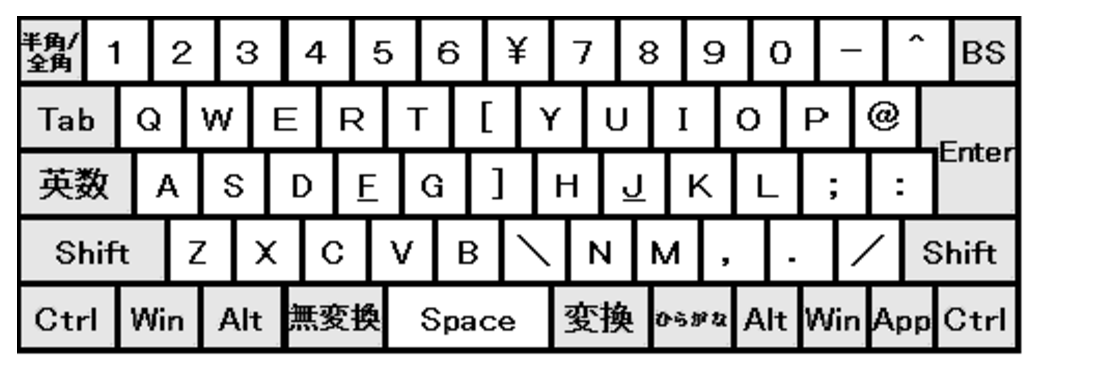
\includegraphics[width=14cm,clip]{res_kouy/migite_1retu_shift.eps}
 \end{center}
 \caption{右手一列シフト}
 \label{migite_1retu_shift}
\end{figure*}

もちろん、親指シフトキーボードを使用すれば、親指キーの位置と大きさは申し分がありません。本格的に親指シフトを使用することにするなら、親指シフトキーボードの使用も選択肢に入ってくるでしょう。

\subsubsection*{BackSpaceの位置は大切}

もう一つ、「親指シフト」とは直接関係はありませんが、親指シフトが入力しやすい理由を挙げます。

親指シフトでは、右手小指ホームポジションの1つ右のキー、つまり\key{:}の位置のキーに\key{BackSpace}が割り当てられています。通常、\key{BackSpace}は文字キーの右上の外れの、かなり遠い位置にあります。しかし、\key{BackSpace}は文章入力を行う中で最もよく使うキーの一つです。どんなに熟練してもタイプミスを無くすのは容易なことではありません。考えながら文章を入力するときは、いま入力した文を消したい場合もあります。そのたびに遠くの\key{BackSpace}を押しに行くというのは大変な労力です。\key{BackSpace}を近くに配置することは、新配列の使用に勝るとも劣らない入力改善効果があります。

また、新配列を習得するという点から見ても、\key{BackSpace}が押しやすいことは重要です。新配列を練習する際は、どうしてもタイプミスが多発します。\key{BackSpace}が押しやすい位置にあれば、タイプミスをしてもすぐに修正できるので、タイプミスを恐れずにどんどん入力することができます。どんどん入力できれば早く慣れることができ、新配列の習得も早くなります。

親指シフトでは、\key{BackSpace}の配置場所が、\key{:}というホームポジションから近い位置に確保されています。親指シフトを使うと、自動的に\key{BackSpace}が押しやすい位置に配置されることなります。これは親指シフトの隠れたメリットです。

親指シフト以外の配列では、\key{BackSpace}の位置は考慮していないものも多くあります。日本語入力配列で\key{BackSpace}の位置を規定するというのも変な話ですから、当然と言えば当然です。しかし、いま書いた通り\key{BackSpace}の位置は日本語入力においてとても大切です。\key{BackSpace}の位置が決められていない新配列を使うとしても――もっと言えば、新配列を使わずローマ字入力やかな入力を使うとしても――\key{BackSpace}を打ちやすい場所に配置することを考えて良いと思います。例えば、親指にシフトキーを配置しない配列を使用するなら、\key{無変換}や\key{変換}は絶好の候補となります。

\subsection{月配列}

月配列は、中指シフトというシフト方式を使用する配列です。通常のシフトキー(\key{Shift})は文字キーの外の、小指で押す位置に配置されています。親指シフトのシフトキーは親指で押す位置に配置されていますが、“文字キーの外に配置されている”という点は通常のシフトキーと同じです。それに対し中指シフトでは、大胆にも文字キーのど真ん中、すなわち中指のホームポジションである\key{D}と\key{K}にシフトキーを配置します。

図\ref{tuki2-263}は月配列の配列図です。各キーの下に書かれている文字は単打で入力される文字です。一方、上に書かれている文字は\key{★}のキー(\key{D}か\key{K})を事前に押していたときに入力される文字です。(親指シフトと異なり、月配列は同時打鍵ではありません。あとで詳しく説明します)


\begin{figure*}
 \begin{center}
   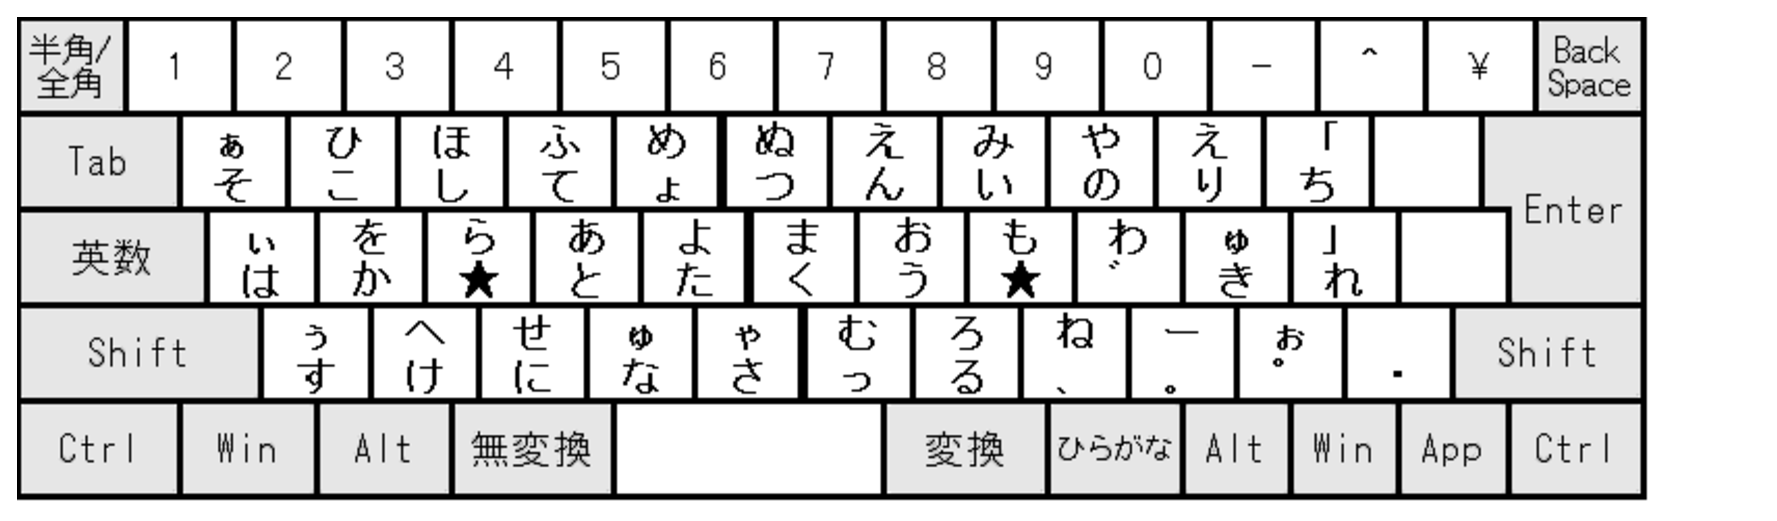
\includegraphics[width=14cm,clip]{res_kouy/tuki2-263.eps}
 \end{center}
 \caption{月配列2-263式配列図}
 \label{tuki2-263}
\end{figure*}

\subsubsection*{中指シフトの利点}

中指のホームポジションにシフトを配置するメリットは、何でしょうか?

まず、シフトキーを特別なキーと考えるのではなく、文字入力に使う1つのキーととらえて、その使用率がどれくらいになるかを考えてみます。

日本語を入力するには61種類の文字を入力する必要があります(記号などを含めるともっと増えます)。また、それらの文字をキーボードの上中下段のうちの32キーを使用して入力することにします。1つのキーに1つの文字を配置するのでは、キーの数が全然足りません。そこで、2つのキーを組み合わせて入力できる文字の種類を増やす「シフト」というシステムが必要になります。

仮に、出現率の高い上位32種類の文字をシフトなし(単打)で入力し、残りの文字をシフトキーを使って入力することにします。すると出現率の低い32~61位の文字の合計出現率は約16.1\%になります。つまり、それだけの回数シフトキーを押す必要があるわけです。
出現率が最も高い文字は「゛」(濁点)で約10.0\%、2位が「い」で約5.6\%、3位が「う」で約5.0\%と続きます。シフトを使用する文字は、これらのトップクラスの出現率の文字と比べても高い率で出現することがわかります。

したがって、シフトキーを特別なキーと考えず、「よく使う“文字”は最も押しやすい位置に配置する」という打ちやすい配列を作る基本的な発想に立って考えると、ほかのどの文字よりも、シフトキーこそ、最も良い位置に配置するべきだ、ということになります。最も押しやすいキーとしては、人差し指と中指のホームポジションが考えられます。しかし、人差し指はもともと担当キー数が(上中下段の3段に限っても)6キーと多いため、使用率があまりにも高い役割を与えるのには向きません。したがって、中指のホームポジションである\key{D}と\key{K}がシフトキーの役割を果たすのに最適なキーということになります。

\subsubsection*{月配列を作ったのは誰か?}

中指シフトという入力方式は、花配列という配列で誕生しました。1999年に冨樫雅文氏が考案した配列で、「風」という漢字変換システムで使用することを想定して作られました。中指シフトを初めて採用し、コンピュータを使用した計算により文字の配置を決定した配列です。

ところで、新JIS配列という配列があります。1986年に制定された配列で、従来のJIS配列(普通のかな入力のこと)とは異なり、最上段(数字段)は使わず上中下段の3段にすべての文字が配置されています。高校教科書や天声人語のデータを使用して、左右交互打鍵が多く、同指異鍵が少なくなるように作られました。実際に新JIS配列が搭載されたワープロも発売されましたが、普及は進まず、1999年に「使用実態がないため廃止」されました。

新JIS配列もなかなか優れた配列だと思うのですが、一つ明確な欠点がありました。それは、通常の小指で押すシフトキーを使用することです(センターシフトも考慮されていましたが、実現しなかったようです)。シフトの使用率は従来のかな入力よりも高いので、小指でシフトキーを押すと小指の使用率がかなり高くなってしまうのです。

「それなら新JIS配列で中指シフトを採用すれば良いのではないか?」、こんな発想が生まれました。どこで生まれたかというと、日本最大の電子掲示板、2ちゃんねるです。
2002年、2ちゃんねるのパソコン一般板に「【ローマ字,仮名,親指?】新JIS配列キーボード」というスレッドが立ちました。当初の話題は新JIS配列の評価や使用法でしたが、しだいに他の配列との比較も語られるようになり、花配列の中指シフトも話題に上がりました。そんな流れの中で「『中指新JIS配列』はどうか?」と提案するレスが書き込まれます。そして実際に中指新JIS配列を試す者が現れ始め、それはだんだんと人数を増していき、試した者から高評価のレスが書き込まれます。

やがて、中指新JIS配列の愛称として「月」が提案されて、次のスレッドのタイトルは「新JIS・月 キーボード配列 2打鍵目」と「月」という名称が入ることになりました。

新JIS配列は中指シフトのために作られた配列ではありませんので、そのまま中指シフト化することはできません。新JIS配列を中指シフト用に改良する必要があります。特に、新JIS配列で中指のホームポジションに配置されていた文字をどうするかが問題になります。

「新JIS配列の良さを残したまま中指シフト化するにはどう配置したら良いか」。スレッド内でさまざまな議論が交わされ、多くの改良案が提案されました。そしてついに、どうやらこれでうまくいったようだという配列が完成します。これを月配列2-263式と呼びます。2-263というのは、新JIS・月配列スレッドの2スレ目の、263番のレスで提案された配列という意味です。その後も改良は進められましたが、2-263式の愛用者は多く、2-263式が月配列の最も標準的な配列という位置づけになっています。

月配列は、新JIS配列と中指シフトという組み合わせの妙が、まず傑出しています。そして、それが生まれたのがインターネットの掲示板で、不特定多数の人の協力で完成したという点が極めて現在的で、新配列の象徴と言える存在だと思うのです。

\subsubsection*{エミュレータなんていらない?}

月配列の中指シフトは「前置シフト」というシフト方式で入力します。親指シフトは同時打鍵でしたが、月配列は同時打鍵ではありません。

前置シフトというのは、「そのキーを押す前にシフトキーを押す。シフトキーを離したかどうかは問わない」というシフト方式です。例えば、月配列で単に\key{J}を押すと「う」と入力されますが、先に\key{D}を押してから\key{J}を押すと(\key{D}を離したかどうかは問わない)「お」と入力されます。

この操作を冷静に考えてみると、キーを押すタイミングはローマ字入力と同じです。ローマ字入力でも、単に\key{A}を押すと「あ」と入力され、\key{K}を押してから\key{A}を押すと「か」と入力されます。月配列もそれと同じことをしています。したがって、月配列は今まで使っていたローマ字入力でのキーを押す感覚で入力できるというメリットがあります。

さらに、「ローマ字入力と同じシステムである」ということから、意外なメリットも生じます。それは「IMEのローマ字カスタマイズで実装できる」ということです。ローマ字カスタマイズというのは、ローマ字のつづりを変更できるIMEの機能です。例えば、通常ローマ字入力では\key{K}の次に\key{A}を押すと「か」と入力されます。この\key{K}と\key{A}の部分を変更できるのです。したがって、\key{S}を押すと「か」と入力されるように設定することも可能なわけです(なお、機能の名称はIMEによって異なります。『Microsoft IME』では「ローマ字設定」、『ATOK』では「ローマ字カスタマイズ」、『Google 日本語入力』では「ローマ字テーブル」という名称です)。

新配列を使う場合の不安点の一つに、「実装できるかどうか」というものがあります。配列エミュレータで実装する場合、いま使っているパソコンでエミュレータが期待通りに動かない可能性もあります。自分のパソコンでは動いても、別のパソコンでは動かないかもしれません。今は動いても将来動かなくなるという不安を完全に払拭することはできません。

この点、月配列はかなり安心です。なぜなら、IMEのローマ字カスタマイズで実装することができるからです。月配列のシフトのシステムはローマ字入力と同じですので、ローマ字カスタマイズを使えばIMEの機能のみで月配列を実装できます。エミュレータを使う必要がありませんから、「実装できない」という心配はかなり少なくなります。

ただし、IMEによってはローマ字カスタマイズに制限がある場合があるので、月配列のすべてを実装することはできないこともあります。その場合、IME用に少しアレンジして実装することになります。『Google 日本語入力』のローマ字カスタマイズは非常に強力ですので、ほぼ制限無く実装することができます。

また、エミュレータを使う場合であっても、同時打鍵などの複雑な操作がないので、エミュレータの選択肢も多く、実装も比較的簡単です。「さまざまな環境で新配列を使用したい」「難しいエミュレータは使いこなせない」と思う人にもおすすめです。

\subsection{AZIK}

今まで紹介した「親指シフト」と「月配列」は、いままで使っていたローマ字入力とはまったく別に、一からかなを配置し直した配列でした。それに対してこれから紹介する「AZIK」は、今まで使っていたローマ字入力はそのまま生かして、その中で入力方法を改善しようという配列です。

\subsubsection*{ローマ字入力拡張配列とは?}

AZIKは、ローマ字入力を拡張して、ローマ字入力では入力しにくい部分を改善する配列です。

例えば、ローマ字入力で「しゃ」と入力する場合は\key{S}\key{Y}\key{A}と入力します。これは当たり前のことのようですが、しかし\ruby{拗音}{ようおん}の入力に3打鍵かかるというのは、合理的ではありません。「じゃ」は\key{J}\key{A}の2打鍵で入力できることを考えれば分かるように、拗音も本来は2打鍵で入力できて良いのです。そこでAZIKでは、\key{X}でしゃ行を入力できることにします。例えば、「しゃ」と入力する場合は\key{X}\key{A}と2打鍵で入力します。しゃ行の拗音はかなり出現率が高いので、これだけでも結構な入力改善効果があります。

ほかにも、AZIKでは次のような拡張入力を使用できます。
\begin{itemize}
 \item \key{;}(\key{L}の1つ右のキー)で「っ」を入力する。ローマ字入力での「っ」の入力方法は、場合によって使うキーが異なるなど変則的です。この入力方法を使うことで、常に分かりやすく入力することができます。
 \item \key{C}でちゃ行の拗音を入力する。(例:\key{C}\key{A}で「ちゃ」と入力する)
 \item \key{Q}で「ん」を入力する。ローマ字入力での「ん」の入力方法は、\key{N}だけで入力できたり、\key{N}\key{N}などと入力しなければならない場合があったりして、変則的です。この入力方法を使うことで常に1打鍵で入力することができます。
 \item \key{:}(\key{L}の2つ右のキー)で「ー」を入力する。「ー」はローマ字入力で唯一最上段を使う文字で、入力しづらい文字です。これをホーム段で入力できるようにします。
\end{itemize}
AZIKではこのような拡張入力を積み重ねることで、ローマ字入力をより打ちやすくなるよう改善しています。

\subsubsection*{ローマ字入力はそのまま使える}

AZIKの拡張入力の重要な点は、このような改良を重ねても、もともとのローマ字入力はほぼそのまま使えるということです。

最初に、\key{X}でしゃ行の拗音を入力できると書きました。しかし、これは「しゃ行の拗音を入力するときは必ず\key{X}を使う」という意味ではありません。もし\key{X}\key{A}でしゃ行の拗音を入力できることを忘れてしまったら、通常通り\key{S}\key{Y}\key{A}と入力することもできます。また、\key{X}というキーは、ローマ字入力ではほとんど使用しません(小書きのかなの入力は\key{L}でもできますので\key{X}を使う必要はありません)。\key{X}でしゃ行を入力できることにしても、もともとのローマ字入力はほぼそのまま使用することができます。

ほかのAZIKの拡張入力を見ても、「っ」の入力に使う\key{;}、「ん」の入力に使う\key{Q}、「ー」の入力に使う\key{:}など、もともとのローマ字入力ではほとんど使わないキーばかりです。

このように、AZIKの拡張入力は、本来のローマ字入力では使わないキーや、キーの組み合わせを使って行います。したがって、AZIKを実装した状態でも、AZIKの拡張入力をまったく使わず、ローマ字入力のように入力することも可能です。ローマ字入力を「変更」して使いやすくするのではなく、本来のローマ字入力を「拡張」することによって使いやすくする。これがAZIKの最大の特徴です。

\subsubsection*{AZIKの覚えやすさ}

AZIKの改良が「拡張」であることのメリットは、ローマ字入力を使ったまま、入力方法を改善できることです。

新配列を覚えることで入力効率を改善することができますが、問題は新配列を覚えるまでの期間をどうするかです。どんな簡単な配列でも、新配列を習得するにはある程度の練習期間が必要です。習得までは文章入力がまともにできません。新配列を使いたいと思っても、この期間のつらさを思ってあきらめてしまう方も多いでしょう。

AZIKならその心配はありません。AZIKなら、今まで使っていたローマ字入力はほぼそのまま使えます。したがって、AZIKを完全に習得していない段階でも、すぐに実際の文章入力で使用することができます。できる範囲で拡張入力を使い、忘れてしまったらローマ字入力の方法で入力すればよいのです。そうやって使っていくうちに慣れて覚えることができます。

そして、AZIKは完全にマスターする必要すらありません。AZIKの拡張入力は、上に紹介した以外にもさまざまなものが用意されています。中にはかなり高度な拡張もあります。しかし、AZIKを使用するのにそれを使いこなさなければならないということはありません。「しゃ行を\key{X}で入力する」「「っ」を\key{;}で入力する」という簡単な拡張入力だけを使うという使用方法でも良いのです。簡単な拡張をまず使ってみて、それで覚えられる自信がついたら次の拡張入力に進むこともできますし、これで十分だと思えばそこまでの段階で使い続けることもできます。そしていつか余裕ができたら、改めて次の拡張入力にチャレンジするということもできるのです。

\subsection{Dvorakローマ字}


\begin{figure*}
 \begin{center}
   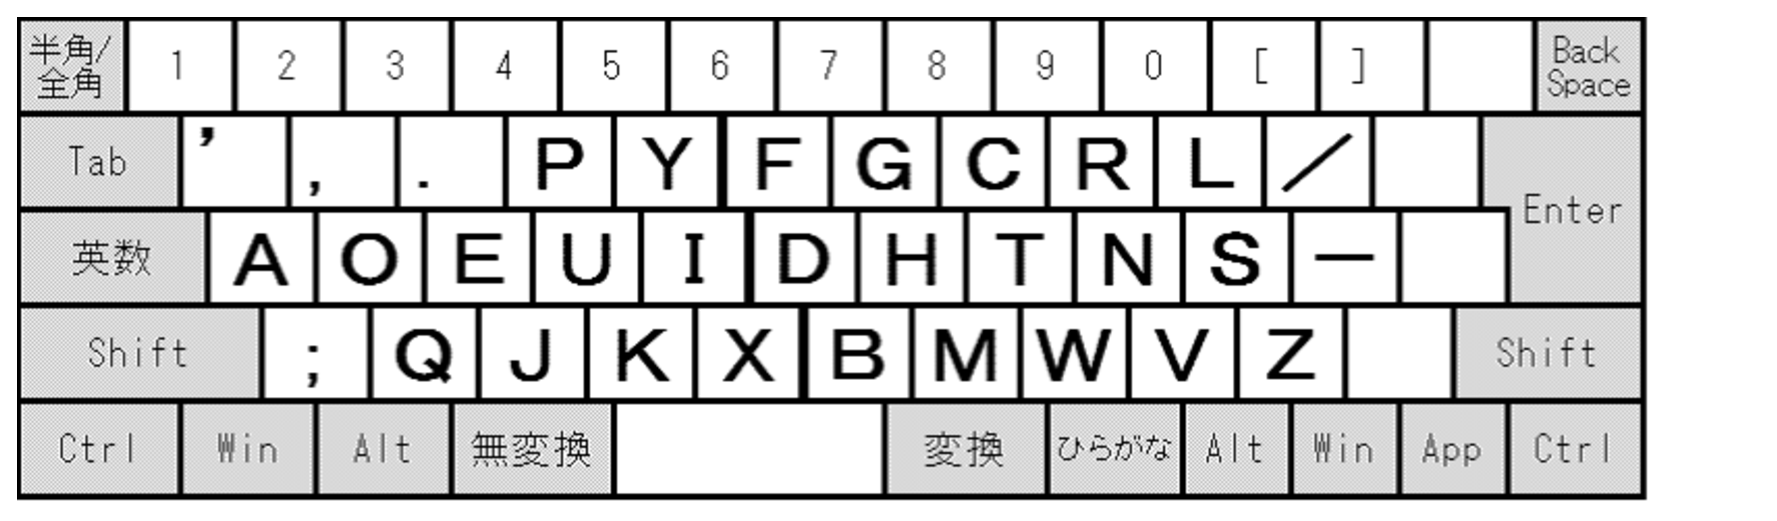
\includegraphics[width=14cm,clip]{res_kouy/Dvorak.eps}
 \end{center}
 \caption{Dvorak配列図}
 \label{Dvorak}
\end{figure*}

\subsubsection*{英語入力も改善しよう}

これまで紹介した新配列は、すべて“日本語での”入力を改善しようとするものでした。一方、英語でも入力方法を改善しようという配列が存在します。一般的に多く使われているアルファベットの配列のことを、キーボードの上段の左から6文字を取って「Qwerty配列」と呼びます。Qwerty配列に代わる配列として有名なのが「Dvorak配列」です。

Dvorak配列の成り立ちは古く、1932年にアメリカで生まれました。考案者のオーガスト・ドヴォラック名前を取ってDvorak配列と呼ばれています。英文でのアルファベットの出現率やキーの打ちやすさを考慮して各文字の配置が決められています。母音がすべて左手のホーム段に配置されているのが特徴。Qwerty配列に比べて交互打鍵率が高く、指の移動距離が短くなります。タイピング速度や快適性の向上、\ruby{腱鞘炎}{けんしょうえん}などの防止に効果があると言われています。

実は、Dvorak配列はローマ字入力をする場合も優れた配列です。というのは、Dvorak配列はローマ字入力の母音である\key{A}\key{I}\key{U}\key{E}\key{O}が左手のホーム段に並べて配置されているからです。QWERTY配列のローマ字入力の欠点は、最もよく使うキーである母音キーが、最も打ちやすい場所には配置されていないことでした。\key{A}が小指のホームポジションにあるだけで、ほかの4キーはすべてホーム段から外れた場所にあります。Dvorak配列なら母音がすべてホーム段にあります。したがって母音を入力するときにホームポジションから指が離れにくく、効率的に入力することができます。

日本語の入力とともに英語の入力も改善したいという方は、Dvorak配列を覚えて両方一気にこれで解決するというのも良いと思います。

\subsubsection*{Dvorakローマ字も拡張しよう}

しかし、当然ながらDvorakもローマ字入力用に作られた配列ではありませんので、Dvorak配列でそのままローマ字入力をしようとすると、いくつか気になる点も出てきます。
代表的なのが、\key{K}が母音と同じ左手側にあることです。このため、か行のかなを入力するたびに左手を続けて使うことになります。特に、「き」と「く」を入力するときに左手の人差し指を続けて使うことになるのが問題です。

この問題の解決策として有名なのは、か行の入力を\key{K}の代わりに\key{C}でできることにするという方法です。感覚的にも、CAで「か」と読めますし、CA・CU・COで「か・く・こ」と入力できるIMEも多いです。慣れれば問題なく入力できるでしょう。

さらに改良点を拡大して、AZIKのような拡張ローマ字入力をDvorak配列にほどこした配列もあります。『DvorakJP』は比較的穏やかな改良。元のDvorak配列から変更点が少なく、なじみやすいと思います。『ACT』は踏み込んだ改良。「AZIK」と同じように簡単な拡張から高度な拡張まで幅広く備え、打ちにくい運指をできる限りなくす大胆な改良を施しています。

これらのDvorak拡張配列は、元にしているDvorak配列自体がローマ字入力に適しているので、英語配列を離れて、単に日本語入力配列として見てもかなり強力です。せっかくDvorak配列を覚えるのなら、日本語入力の方は最初からDvorak拡張配列を覚えるというのも良いでしょう。

\subsection{けいならべ}


\begin{figure*}
 \begin{center}
   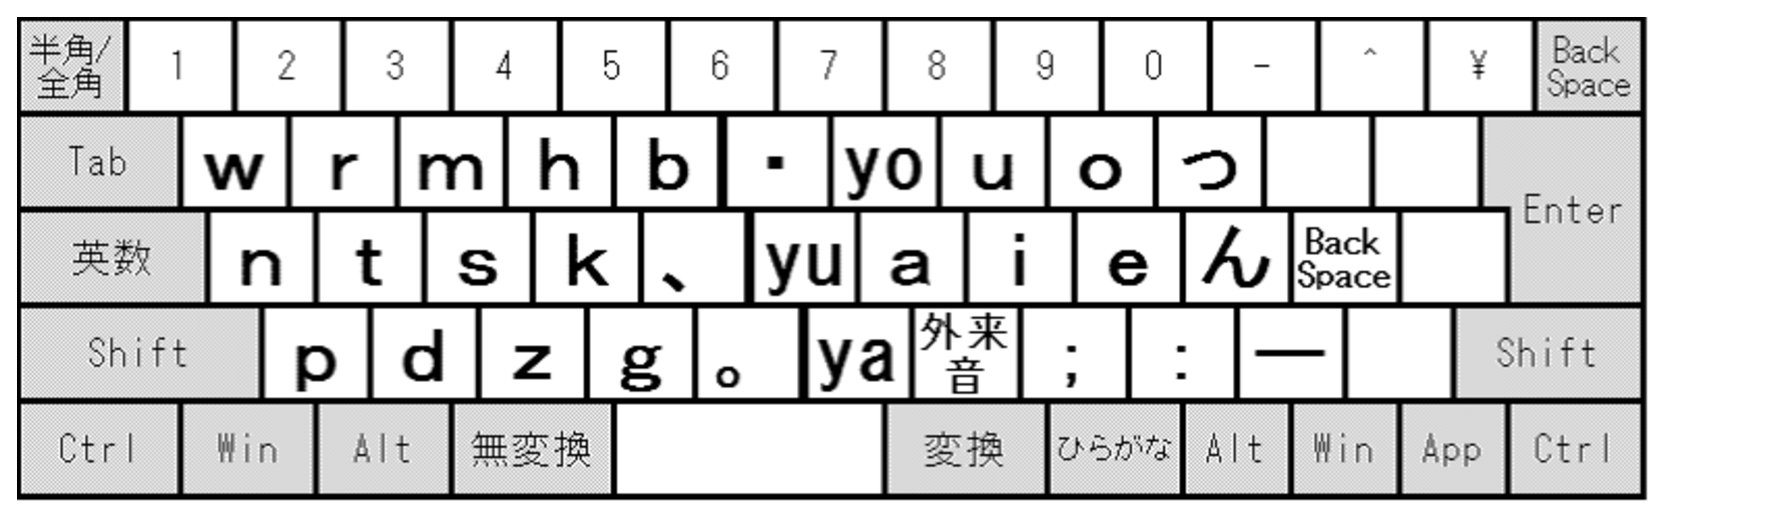
\includegraphics[width=14cm,clip]{res_kouy/keinarabe.eps}
 \end{center}
 \caption{けいならべ配列図}
 \label{keinarabe}
\end{figure*}

\subsubsection*{五十音順行段系配列}

けいならべは、覚えやすさに重点をおいた行段系配列です。行段系というのは、1つの文字を基本的に子音と母音の2打鍵で入力する配列のことです。かなの五十音表を利用して、子音と母音を組み合わせることで1つのかなを入力します。ローマ字入力も行段系配列の一種です。

そして、けいならべでは子音と母音が左右にはっきり分かれて配置されています(図\ref{keinarabe})。左手が子音キー担当、右手に母音キー担当です。

さらに、そのキーの並び方もかなり規則的です。子音を入力するキーは左手人差し指のホームポジションである\key{F}を起点として、そこから左にか行、さ行、た行、な行の順番。上段に移って\key{R}からは行、ま行、ら行、わ行の順番となっています。これはおなじみの五十音順と同じ順番です(なお、けいならべではや行の子音キーはありません。あとで詳しく説明します)。さらに濁音を入力するキーも、が行、ざ行、だ行のキーは、その清音のキーのすぐ下に配置されています。母音も、やや変則的ではありますが、右手のホームポジションである\key{J}を起点としてあいうえお順で並べられています。

このように、けいならべではなじみ深い五十音の順番を利用して覚えられるように作られています。これならすぐにでも覚えることができるでしょう。

\subsubsection*{左右交互打鍵とアルペジオの威力}

「確かにほかの配列より覚えやすそうではあるけど、行段系ということは基本的に1つのかなの入力に2打鍵かかる。これでは習得しても十分な入力改善効果は得られないのでは?」と思う方もいるかもしれません。確かに、けいならべの打鍵数は、ローマ字入力よりは少ないものの、1打鍵で1文字入力できるかな系の配列と比べるとかなり多くなります。打鍵数が減らないのでは改善効果も大したことはないだろう、と高をくくられるかもしれません。しかし、けいならべは、入力効率改善効果も決して侮ることはできないのです。

けいならべが入力しやすい第一の理由は、基本的に左右交互打鍵で入力できることです。
左右交互打鍵というのは、左手でキーを打ったら次は右手、右手でキーを打ったら次は左手というように、左右の手を交互に使って打鍵することです。これは入力しやすい入力方法です。なぜなら、一方の手でキーを打っている間に、もう一方の手はキーを押す準備をすることができるからです。

けいならべでは子音を左手で、母音を右手で入力します。行段系の入力方法では基本的に子音と母音が交互に出てきますので、必然的に左右交互打鍵で入力できるのです。

もちろん、左右交互打鍵では入力できない部分もあります。例えば、連母音の部分です。連母音というのは、ローマ字で母音が連続して出現する部分のことです。例えば、「かい」という文字を入力するときは\key{K}\key{A}\key{I}と入力します。母音のAとIが連続していますから、この部分は連母音ということになります。けいならべの母音はすべて右手で入力しますから、連母音の部分は必然的に同じ手を続けて使うことになります。

しかし、むしろこの連母音こそが、けいならべの入力しやすさの真骨頂といえる部分です。その秘密は、連母音の偏りと、連母音をアルペジオで入力できることです。

連母音の出現率は、かなの出現率と同じようにに大きな偏りがあります。母音は5種類ですから、連母音は全部で25種類あります。そのうち出現率の高いai、ei、ouの3種類の連母音で全体の約55.3\%を占めます。その3種類の連母音を口に出してみると、多く使う音であることを感じられると思います。特に漢字の音読みで多く使われます。

けいならべでは、この出現率の高い3つの連母音をアルペジオで入力できるようにしてあります。アルペジオというのは、「片方の手で続けてキーを押す場合に、非常に押しやすい連接」のことです。例えば\key{K}→\key{J}と打鍵する場合がアルペジオです。実際にキーを押してみると、この2キーを打鍵する場合は速く楽に打鍵できることが感じられると思います。けいならべでは、連母音aiは\key{J}→\key{K}、eiは\key{L}→\key{K}、ouは\key{O}→\key{I}と、すべてアルペジオで入力できるように配置してあります。けいならべの母音は、子音に比べるとやや変則的な順番で並んでいますが、それは連母音をアルペジオで打てるようにするためです。

基本は左右交互打鍵、出現率の高い連母音はアルペジオで入力。この2つの工夫により、けいならべは覚えやすい五十音順配列でありながら、高い入力改善効果を実現しています。

\subsubsection*{やゆよの母音化とは?}

もうひとつ、けいならべの大きな特徴があります。それは、「やゆよ」を母音化して扱っていることです。

通常のローマ字入力では、母音は「aiueo」の5種類です。「a」は単打で「あ」を入力します。子音「k」と母音「a」の組み合わせで「か」を入力します。「やゆよ」を母音化するというのは、「ya、yu、yo」を「a、i、u、e、o」と同じ扱いにするということです。したがって、「ya、yu、yo」を単打で入力できるキーが存在します。けいならべ配列図(図5-6)の\key{N}\key{H}\key{U}のキー、下から順番に「ya」「yu」「yo」と並んでいる部分がそれです。これらのキーを単打で押すと、「やゆよ」が入力されます。一方、子音キーを押した後に「ya、yu、yo」を押すと、拗音を入力します。例えば、「k」のキーを押してから「ya」のキーを押すと「きゃ」を入力します。拗音というのは、子音とや行の組み合わせですべて表現することができるのです。

図\ref{keinarabe_50on}はやゆよを母音扱いした五十音表です。やゆよを母音扱いするというと奇異に思えるかもしれませんが、表を隙間なく埋めた上で拗音も規則的に取り込めるので、むしろ通常の五十音表より分かりやすくまとまっていると思います。


\begin{figure*}
 \begin{center}
   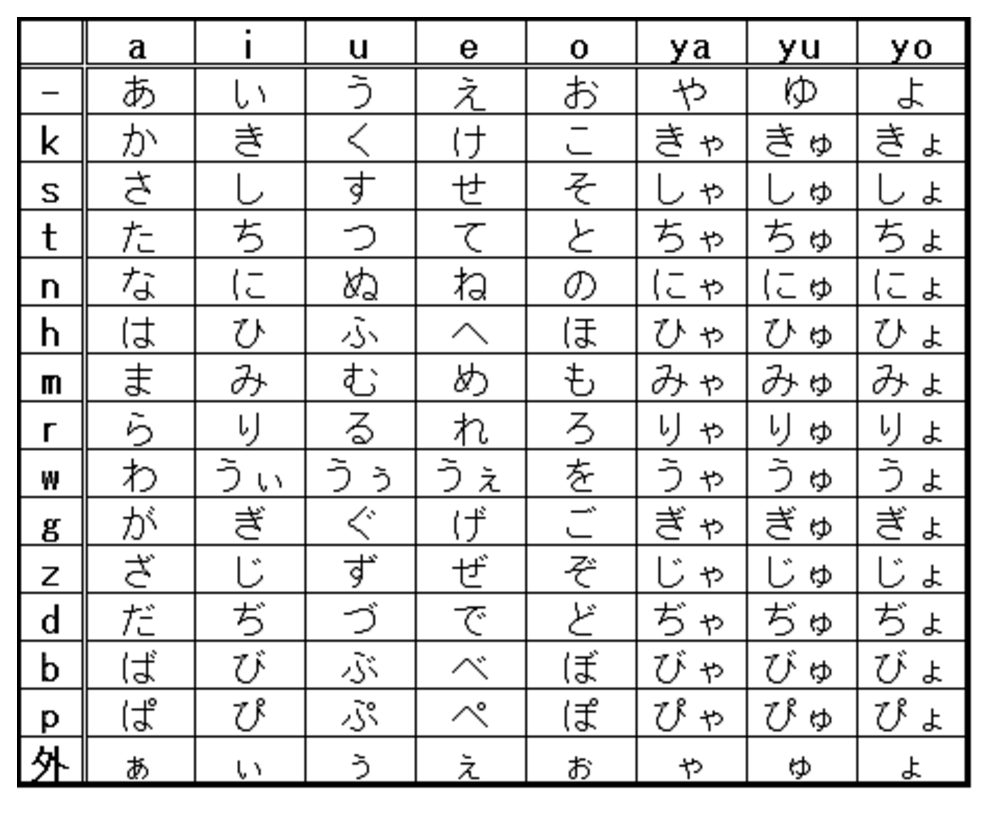
\includegraphics[width=14cm,clip]{res_kouy/keinarabe_50on.eps}
 \end{center}
 \caption{やゆよを母音扱いした五十音表}
 \label{keinarabe_50on}
\end{figure*}

やゆよを母音化するメリットは2つあります、まず、拗音をすべて2打鍵で入力できることです。通常のローマ字入力では拗音の入力は多くは3打鍵ですので、その分打鍵数を減らすことができます。通常のローマ字入力でも、じゃ行の拗音だけは2打鍵で入力できるので、じゃ行だけは入力しやすいと感じられている方も多いと思います。それがすべての拗音に拡大されるのは大きなメリットです。

もう一つは、や行の連母音の入力がしやすいことです。先ほど頻出する連母音をai、ei、ouと3つ挙げました。しかし、実はやゆよを母音扱いすることにすると、you(ょう)という連母音も非常によく出現する連母音となります。「ょう」という文字の連なりは、2文字の連なりの中では断トツです。けいならべでは、この連母音youも\key{U}→\key{I}のアルペジオで入力できるようになっています。「やゆよ」が(上からではなく)下から順番に並んでいるのは、\key{yo}と\key{u}をアルペジオで入力できるようにするためです。

通常の連母音3種に加えて、拗音の連母音youもアルペジオで入力できることにより、けいならべは行段系の入力方法でありながら、打鍵数を意識させないスピード感のある入力をすることができるのです。
